\subsection{Linear Classifier}
\begin{quote}
"e.g. cost/error function, decision boundary and training method"
\end{quote}


The goal of linear classification is to take an input vector with multiple x values and assign it to one of multiple classes K. This can be done with one or more linear decision boundaries. The first way to classify is called the one-vs-one linear classifier. This works for 2 classes as seen in figure \ref{onevsone1}. If multiple clusters of x belonging to more than 2 classes are present we get ambiguous regions as one class might appear to be two different classes. An example of this can be seen in figure \ref{onevsone2}.
\begin{figure}[H]
\centering
\begin{minipage}[b]{0.5\textwidth}
\centering
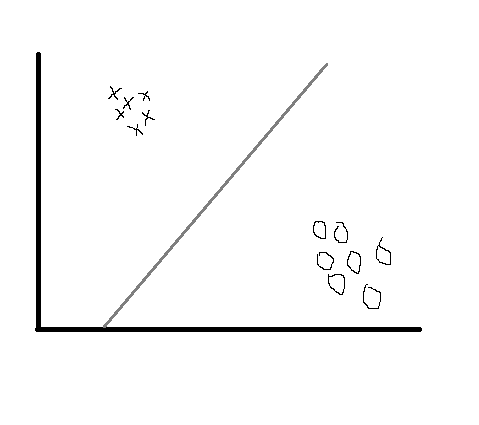
\includegraphics[scale=0.5]{billeder/onevsone1}
\caption{One-vs-one linear classifier for 2 classes}
\label{onevsone1}
\end{minipage}%
\begin{minipage}[b]{0.5\textwidth}
\centering
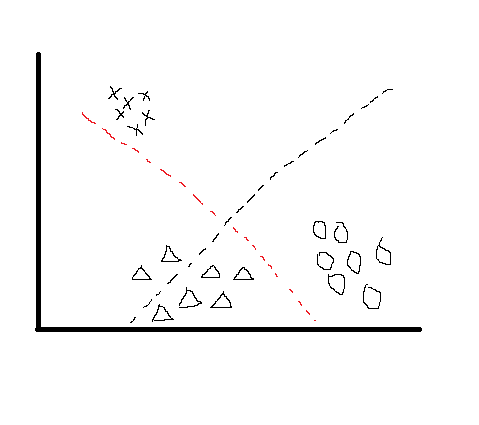
\includegraphics[scale=0.5]{billeder/onevsone2}
\caption{One-vs-one linear classifier for 3 classes}
\label{onevsone2}
\end{minipage}
\end{figure}
Another way to classify  the 3 classes seen in figure \ref{onevsone2} could be to utilise 1-of-k classification. This can be seen in figure \ref{oneofk1}. The 1-of-k classifier  has no ambiguity in this case.
\begin{figure}[H]
\centering
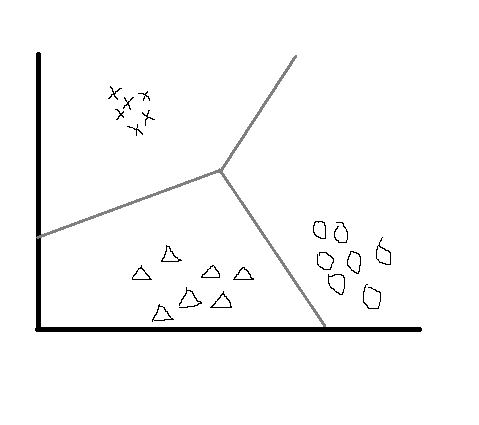
\includegraphics[scale=0.5]{billeder/oneofk1}
\caption{1-of-k linear classifier for 3 classes}
\label{oneofk1}
\end{figure}
In math terms the one-vs-one can be written as:
\begin{equation}
y(\textbf{x})=\tilde{\textbf{w}}^T\tilde{\textbf{x}}
\end{equation}
This is prone to ambiguity for more than 2 classes. We know that the ambiguity issue can be avoid by using the form:
\begin{equation}
y_k(\textbf{x})=\textbf{w}_k^T\textbf{x}+\omega_{k0}
\end{equation}
and choosing the value of x to be a part of class k if $y_k(\textbf{x})>y_{m}(\textbf{x})$ for all $m \neq k$. This leads to decision boundaries corresponding to the 1-of-k classifier.

How we use it\\

Intermediate result\\

%------------------------------------------------